\documentclass[10pt,a4paper]{article}
\usepackage[margin=2.1cm]{geometry}
\usepackage{amsmath,amssymb}
\usepackage{graphicx}
\usepackage{booktabs}
\usepackage{xcolor}
\usepackage{microtype}
\usepackage[font=small,labelfont=bf]{caption}
\usepackage[hidelinks]{hyperref}
\usepackage{natbib}
\setlength{\parskip}{0.35em}
\setlength{\parindent}{0pt}
\newcommand{\nodetect}{40}
\newcommand{\outsideprior}{42}

\newcommand{\opa}{6}
\newcommand{\opb}{-10}
\newcommand{\opmismatch}{0}

\makeatletter\newcommand{\tabinput}[1]{\@@input #1 }\makeatother

% ---- replace before release -------------------------------------------------
\newcommand{\authorname}{d3st}
\newcommand{\repourl}{https://github.com/3cthulhu3/argus-autonomy}
% -----------------------------------------------------------------------------

\title{\textbf{Active Wildfire-Front Estimation for a Single UAV}\\[0.3em]
\large Satellite prior, thermal sensing and information-rate planning under safety constraints}
\author{\authorname\\ \small Argus Aegis project\\ \small \url{\repourl}}
\date{Technical report, v1.1 $\cdot$ October 2026}

\begin{document}
\maketitle

\begin{abstract}
\noindent
Early confirmation of a wildfire is a problem of \emph{active estimation}. A satellite hotspot product says roughly where a fire was some minutes ago; an onboard thermal camera says precisely, but noisily, what lies beneath the aircraft right now; and the endurance budget is fixed. We study a single UAV that fuses both sources in a per-cell Bayesian occupancy filter, propagates the belief through its own fire-spread model, and plans with a greedy information-rate objective. A geofence and a return-to-base monitor may override any move. In 100-seed Monte Carlo simulation, the planner is compared with a full-map lawnmower and with a lawnmower restricted to the satellite hotspot box. Relative to the stronger baseline, it cuts the median time to first confirmation by 45\,\% (1.8 vs.\ 3.3\,min) and halves the median perimeter error (18 vs.\ 35\,m on a 25\,m grid). There are no safety violations in 900 missions. We also report two failure modes. The first is an idealised calm-air spread model; the planner still leads under it, but its prediction step alone then recovers only about a third of the burnt area. The second is misspecification of the satellite prior, where the greedy planner fails catastrophically more often than a prior-blind sweep. A one-parameter tempering of the prior removes most of these failures, which marks prior robustness as the open problem. Version~1.1 (Section~\ref{sec:v11}) addresses a third failure: persistent non-fire heat sources, which the occupancy filter confirms as fire on every decoy cue. A sequential test between a spreading-fire model and a static-world model turns growth into evidence; thresholds chosen on one seed set and reported on another give 1.2\,\% false alerts on decoy cues (95\,\% upper bound 2.1\,\%), 0.2\,\% dismissed fires and an unchanged median alert time of 2.2\,min, at the cost of 1.5\,min more to dismiss a decoy.
\end{abstract}

\section{Problem}
The world is an $n\times n$ grid ($n=64$, cells of 25\,m, so 1.6\,km square). Each cell $i$ has a hidden binary state $X_i^t\in\{0,1\}$, \emph{affected} (burning or burnt) or not. $X^t$ is monotone in $t$. At launch the vehicle holds a prior from a satellite hotspot product. At every tick (10\,s) it moves at most 4 cells and observes a $7\times7$ footprint. The questions are:
\begin{enumerate}\setlength{\itemsep}{0pt}
\item How soon is the fire \emph{confirmed}, i.e.\ some truly affected cell reaches posterior $\ge 0.95$?
\item How well is the perimeter localised when the vehicle lands (F1 of the thresholded map, perimeter distance)?
\end{enumerate}
Two constraints hold throughout: never enter the no-fly zone, and always keep enough endurance to return to base with a reserve. The endurance is 180 ticks (30\,min).

\section{Simulation model}
\paragraph{Fire.} A stochastic cellular automaton, in the spirit of \citet{alexandridis2008}, steps once per minute. A burning neighbour $j$ ignites an unburnt cell $i$ in direction $d_{ji}$ with probability
\begin{equation}
q_{ji} = p_0\, \phi_i\, \frac{\exp\!\big(k\cos\angle(d_{ji}, w)\big)}{\lVert d_{ji}\rVert},
\qquad
P(\text{ignite } i) = 1-\prod_{j\in\mathcal N(i)}\big(1-q_{ji}\,\mathbf{1}[j\text{ burning}]\big),
\label{eq:spread}
\end{equation}
with $p_0=0.1$ and wind gain $k=1.6$. The wind direction $w$ is random per seed, and $\phi$ is a spatially correlated fuel field in $[0.3,1.3]$. Cells burn for 8 steps and then burn out. The fire is ignited 15\,min before launch.

\paragraph{Satellite prior.} The truth is aggregated into $8\times8$-cell pixels (200\,m), loosely modelled on 375\,m VIIRS active-fire pixels \citep{schroeder2014}. A pixel is flagged if at least 5\,\% of it is affected. The overpass is $6$\,min old at launch and carries a geolocation error of $\mathcal N(0,2^2)$ cells. The per-cell prior is 0.25 in flagged pixels, 0.02 in the surrounding ring and 0.002 elsewhere.

\paragraph{Sensor.} A nadir thermal camera covers a $7\times7$-cell footprint (175\,m), with independent per-cell detections: $P(z{=}1\mid X{=}1)=p_d=0.85$ and $P(z{=}1\mid X{=}0)=p_f=0.03$.

\section{Estimator}
\paragraph{Update.} In log-odds $\ell_i=\log\frac{b_i}{1-b_i}$, the Bayes update for an observed cell is exact under the sensor model:
\begin{equation}
\ell_i \leftarrow \ell_i + z_i\log\frac{p_d}{p_f} + (1-z_i)\log\frac{1-p_d}{1-p_f}.
\end{equation}

\paragraph{Prediction.} Once per fire step the belief is pushed through the estimator's own version of \eqref{eq:spread}. That version has a homogeneous fuel $\bar\phi=0.8$ and, depending on the condition, the true or a calm-air wind. Under a mean-field (independent-cell) approximation,
\begin{equation}
b_i' = b_i + (1-b_i)\Big(1-\prod_{j}\big(1-\hat q_{ji}\, s_j\big)\Big),\qquad
s_j = \big(b_j - b_j^{(t-8)}\big)\,\mathbf{1}[b_j\ge \gamma].
\label{eq:predict}
\end{equation}
Here $s_j$ is the probability that $j$ became affected recently enough to still be burning. The gate $\gamma=0.5$ is a deliberate departure from plain mean-field. Without it, diffuse low-probability mass sees ``fresh'' neighbours everywhere and grows exponentially: started from the true state, ungated prediction over-predicts the burnt area $4.7\times$ after 30\,min, and with a diffuse prior the map saturates (Table~\ref{tab:cal}). The gate trades this blow-up for systematic under-prediction between observations.

\section{Planning and safety}
\paragraph{Information rate.} For a cell with belief $b$, the mutual information between state and one observation is
\begin{equation}
I(b) = H_2\big(b\,p_d+(1-b)p_f\big) - b\,H_2(p_d) - (1-b)\,H_2(p_f),
\end{equation}
where $H_2$ is the binary entropy. The expected gain of a footprint centred at $c$ is $G(c)=\sum_{i\in F(c)} I(b_i)$, computed for all $c$ at once with a box filter. The planner chooses
\begin{equation}
c^\star = \arg\max_{c\,\in\,\mathcal C_{\text{safe}}} \frac{G(c)}{\lceil D(x,c)/v\rceil + \tau},\qquad \tau = 1,
\end{equation}
re-planning every 2 ticks, where $D$ is the geodesic distance around the no-fly zone. This is a one-step greedy policy in the tradition of information-based exploration \citep{bourgault2002, hollinger2014}. The prediction step creates uncertainty exactly where the front is expected to advance, so the planner tracks the perimeter without any explicit front model.

\paragraph{Safety monitor.} Motion follows 8-connected geodesic paths, with no corner-cutting into the no-fly zone. A waypoint is admissible only if
\[
\lceil D(x,c)/v\rceil + \lceil D(c,\text{base})/v\rceil \le T_{\text{rem}} - T_{\text{res}} - 2,
\]
with a reserve $T_{\text{res}}=6$ ticks. Independently of the planner, the monitor forces return-to-base when the remaining endurance only just covers the way home. The baselines are subject to the same monitor. The monitor is a checkable runtime invariant on the grid, not a formal guarantee for continuous dynamics; extending it in that direction, e.g.\ with reachability analysis, is future work.

\section{Experimental protocol}
There are three conditions, each with 100 seeds (0--99) and three planners. For a given seed, the fire, wind, fuel and satellite prior are drawn from independent random streams, so every planner faces \emph{the same} fire.
\begin{itemize}\setlength{\itemsep}{0pt}
\item \textbf{nominal}: the estimator's model has the true wind; the prior is as above.
\item \textbf{wind-mismatch}: the truth is wind-driven, but the estimator assumes calm air ($k=0$).
\item \textbf{degraded-prior}: the overpass is 12\,min old and the geolocation error is $\mathcal N(0,6^2)$ cells.
\end{itemize}
The baselines are a full-map boustrophedon (\emph{lawnmower}) and a boustrophedon over the bounding box of the flagged pixels plus their ring (\emph{prior-lawnmower}). The second is the strong baseline, since it uses the same prior information as the planner. Paired differences use the Wilcoxon signed-rank test. All tables are generated from \texttt{results/*.json} by \texttt{experiments/make\_report\_tables.py}.

\section{Results}
\begin{table}[h]
\centering\small
\caption{Benchmark, 100 seeds per row. Confirmation times are medians with [IQR]. The ``50\,\% confirmed'' column gives the median time until half of the true affected area has posterior $\ge 0.95$, with the number of runs that reached it in parentheses. F1 is the mean $\pm$ 95\,\% CI at landing; the perimeter error is a median.}
\label{tab:main}
\setlength{\tabcolsep}{5pt}
\begin{tabular}{lccccc}
\toprule
Planner & 1st confirm.\ (min) & 50\,\% confirmed (min) & F1 & Perim.\ err.\ (m) & False conf.\\
\tabinput{tables/main.tex}
\bottomrule
\end{tabular}
\end{table}

\begin{table}[h]
\centering\small
\caption{Info-rate minus prior-lawnmower, paired on identical seeds. Each block gives the median difference, the share of seeds where info-rate is better, and the Wilcoxon $p$-value.}
\label{tab:paired}
\setlength{\tabcolsep}{4pt}\footnotesize
\begin{tabular}{lccccccccc}
\toprule
& \multicolumn{3}{c}{1st confirmation} & \multicolumn{3}{c}{F1} & \multicolumn{3}{c}{Perimeter error}\\
\cmidrule(lr){2-4}\cmidrule(lr){5-7}\cmidrule(lr){8-10}
Condition & $\Delta$ & better & $p$ & $\Delta$ & better & $p$ & $\Delta$ & better & $p$\\
\midrule
\tabinput{tables/paired.tex}
\bottomrule
\end{tabular}
\end{table}

\begin{figure}[h]
\centering
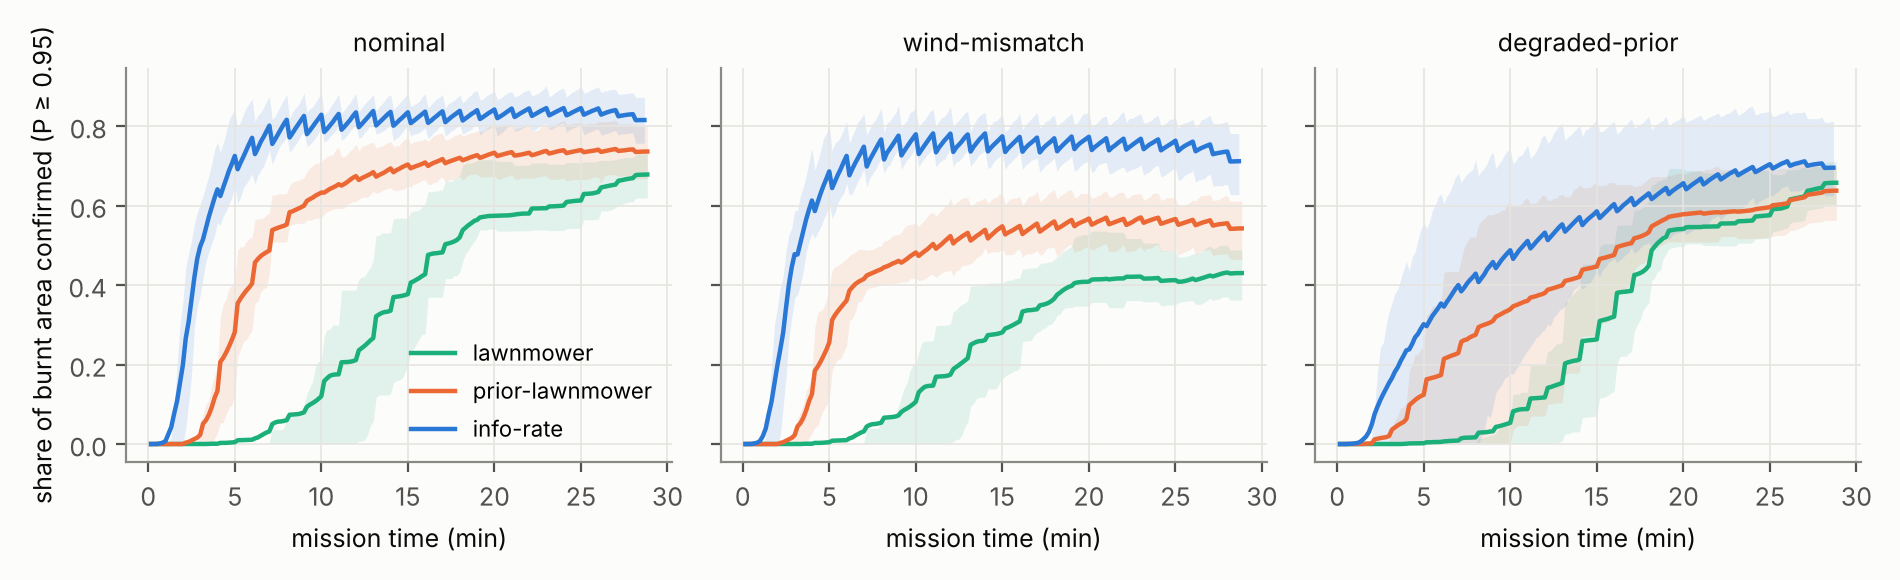
\includegraphics[width=\linewidth]{../../media/recall_vs_time.png}
\caption{Share of the true affected area that is confirmed ($b\ge0.95$), mean with interquartile band. The saw-tooth comes from the fire step: every minute the true area grows and newly affected cells are not yet confirmed.}
\label{fig:recall}
\end{figure}

In the nominal condition the information-rate planner confirms the fire in a median 1.8\,min, against 3.3\,min for prior-lawnmower and 9.4\,min for the full lawnmower. It is faster in 99 of 100 paired seeds, and it also maps the fire better (Table~\ref{tab:main}, Fig.~\ref{fig:recall}). Its median perimeter error of 18\,m is below one grid cell. All 900 missions ended at base with at least 7 ticks of reserve, and no geofence violation occurred. Figure~\ref{fig:snap} shows a representative run; it is the seed whose F1 is the median, not a hand-picked one.

\begin{figure}[h]
\centering
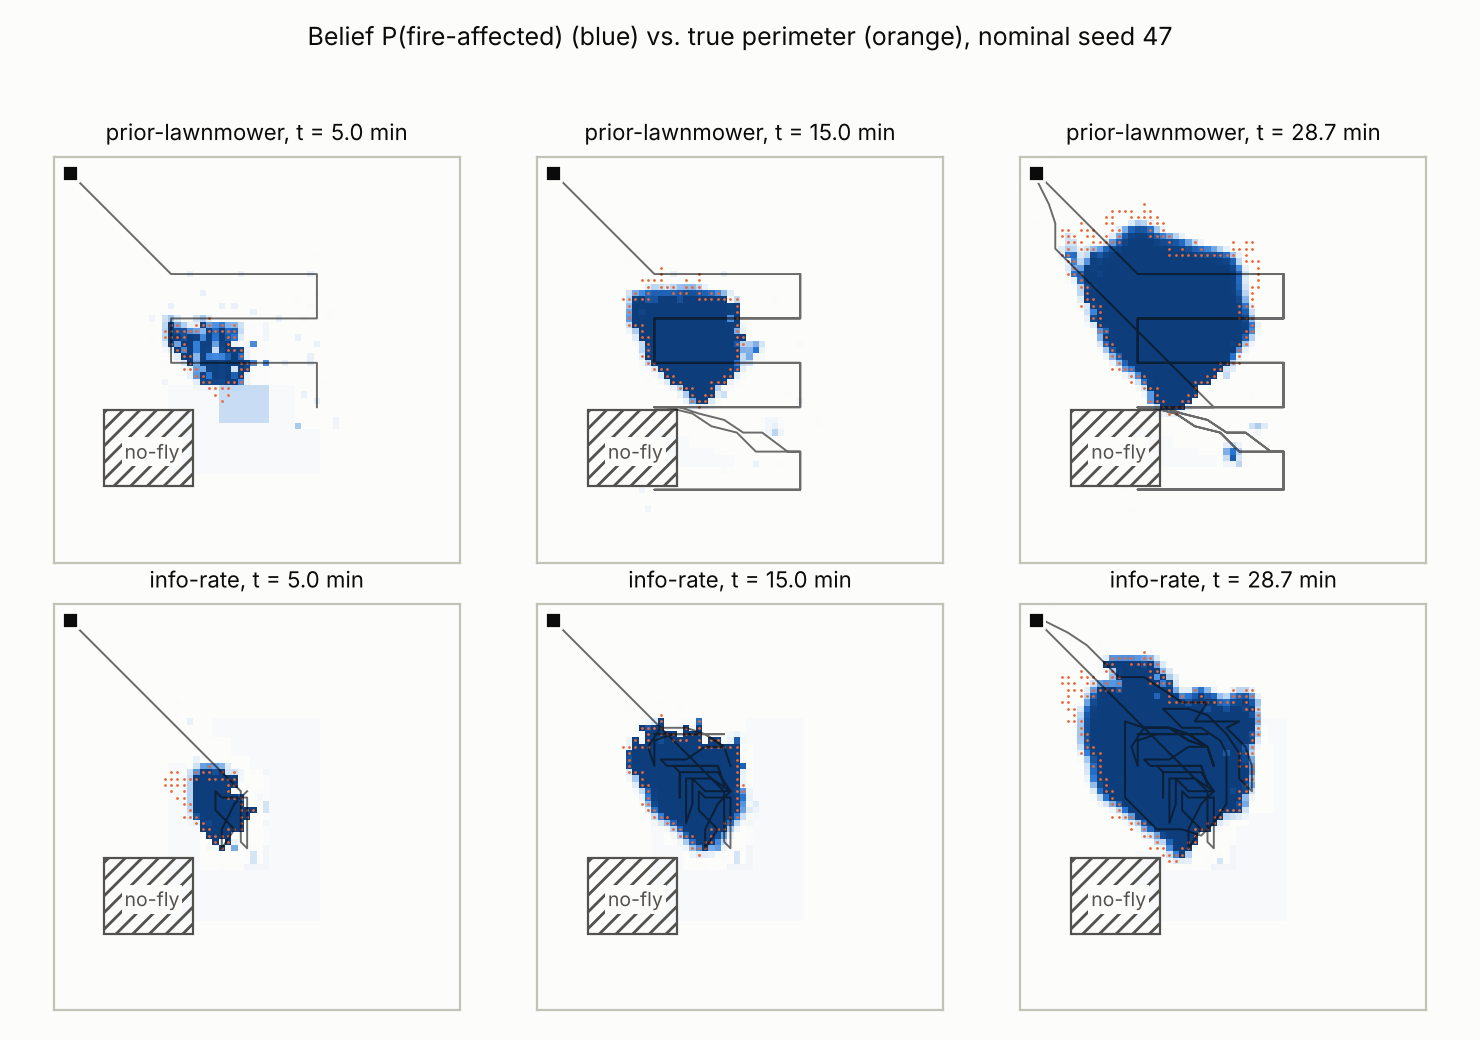
\includegraphics[width=0.86\linewidth]{../../media/snapshot.png}
\caption{Seed 47, the median-F1 nominal run. Belief (blue), true perimeter (orange dots) and trajectory. Prior-lawnmower spends its first minutes sweeping the hotspot box; info-rate goes straight to the most uncertain footprints and then patrols the advancing front.}
\label{fig:snap}
\end{figure}

\section{Failure analysis}
\paragraph{Spread-model mismatch.} Table~\ref{tab:cal} isolates the prediction step. Each run starts from the true state and propagates for 30\,min with no observations. With the true wind, the gated filter recovers 66\,\% of the burnt area; with the calm-air assumption it recovers 35\,\% (IoU 0.28). In closed loop (Table~\ref{tab:main}, \emph{wind-mismatch}), info-rate loses 0.053 F1 and prior-lawnmower loses 0.106. The planner is therefore robust here because it re-observes the front often, not because its model is good. The mismatch shows up instead as an expanding gap behind the downwind front during the last ten minutes (Fig.~\ref{fig:recall}, middle panel).

\begin{table}[h]
\centering\small
\caption{Prediction-only calibration, 50 seeds, medians. Area ratio = predicted ($b\ge0.5$) / true affected area.}
\label{tab:cal}
\begin{tabular}{lcccccc}
\toprule
& \multicolumn{2}{c}{10 min} & \multicolumn{2}{c}{20 min} & \multicolumn{2}{c}{30 min}\\
\cmidrule(lr){2-3}\cmidrule(lr){4-5}\cmidrule(lr){6-7}
Variant & ratio & IoU & ratio & IoU & ratio & IoU\\
\midrule
\tabinput{tables/calibration.tex}
\bottomrule
\end{tabular}
\end{table}

\paragraph{Prior misspecification.} In the \emph{degraded-prior} condition, the overpass detects nothing in \nodetect{} of 100 seeds. In \outsideprior{} seeds, no part of the fire lies inside the flagged pixels or their ring. Info-rate still has the best mean F1, but its distribution is bimodal: 13 runs end with F1 $<0.7$, against 7 for prior-lawnmower and 2 for the prior-blind lawnmower. The mechanism is visible in the gain map. Cells outside the prior carry $b=0.002$, and their mutual information is about 65 times lower than that of a flagged cell, so a greedy objective never pays the travel cost to look there. Table~\ref{tab:temper} sweeps the background prior. At 0.01, catastrophic runs drop from 13 to 3, with no loss in the nominal condition. At 0.05 the background mass itself starts to spread through the prediction step, and both conditions degrade.

\begin{table}[h]
\centering\small
\caption{Tempering the background prior, info-rate, 100 seeds.}
\label{tab:temper}
\begin{tabular}{lccccc}
\toprule
Condition & Background prior & F1 (mean) & Runs with F1 $<0.7$ & 1st confirm.\ (min) & False confirm.\\
\midrule
\tabinput{tables/tempering.tex}
\bottomrule
\end{tabular}
\end{table}

The tempering works, but it is a single hand-tuned scalar. It encodes ``trust the satellite less'' without saying how much less, or how that should depend on the overpass age and geolocation quality. A principled treatment would plan against a set of plausible priors rather than a point estimate, and would quantify the value of exploring outside the prior.

\section{Decoys and a calibrated decision (v1.1)}\label{sec:v11}
\paragraph{The failure.} The sensor model above treats false alarms as independent per look. A persistent non-fire heat source, such as a sunlit rock or a contained burn, answers ``hot'' on every pass, and under that model repeated hot answers are exactly the evidence that confirms a fire. With three static decoys outside the satellite cue, at least one decoy cell is confirmed as fire in 50 of 100 nominal missions. When the cue itself is a decoy, the v1.0 filter confirms it in every mission (Table~\ref{tab:ladder}). Persistence is the decoy's signature, not the fire's; what distinguishes a fire is that it spreads.

\paragraph{Model and test.} Each cell takes one of four classes: empty, fire, \emph{warm} decoy (responds less often than fire) and \emph{hot} decoy (responds exactly like fire at any instant). Two categorical filters run in parallel. $H_1$ (a spreading fire exists) propagates fire mass with the gated prediction~\eqref{eq:predict}; $H_0$ (nothing spreads) is a static world that explains the satellite cue with decoys. Before each update, each filter gives the predictive likelihood of the incoming footprint, and the posterior log-odds
\[
\Lambda_t=\log\tfrac{\pi}{1-\pi}+\textstyle\sum_{s\le t}\big[\log p(z_s\mid H_1,\text{past})-\log p(z_s\mid H_0,\text{past})\big]
\]
is a Bayesian sequential probability ratio statistic \citep{wald1945}. The mission ends in ALERT at the first $t$ with $\Lambda_t\ge a$, in CLEAR at the first $t$ with $\Lambda_t\le b$, or UNDECIDED at endurance. $H_1$ is penalised every time its predicted spread fails to appear, so growth becomes evidence without a hand-written ``is it growing?'' rule. A stopping rule, the \emph{CLEAR gate}, forbids CLEAR until every flagged satellite pixel has been seen. Three planners share the test: info-rate search on $P(\text{any heat})$ (M1); an active-hypothesis-testing rule that maximises the expected drift of $\Lambda$ \citep{chernoff1959, naghshvar2013} (M2); and M2 plus a close-look action, a two-tick hover with a radiometric reading that separates warm decoys from fire but, deliberately, not hot decoys (M3).

\paragraph{Protocol.} Three scenario families share the v1.0 world: A, fire plus decoys; B, decoys only, conditioned on the satellite flagging one (the false-alert family); C, fire only (the v1.0 regression). Every free choice after the first milestone was screened on seeds 5000 and above, and each milestone's expectations were committed before it ran. For the thresholds, every mission flies to endurance without deciding and logs $\Lambda_t$; because the pre-decision policy is independent of $(a,b)$, the decision of every pair is a first-passage time of one run. The operating point was chosen on selection seeds (B 0--999, A and C 0--499) as the pair with the fewest dismissed fires among those with an upper 95\,\% false-alert bound $\le 2\,\%$ and $\le 5\,\%$ undecided missions, and reported on held-out seeds (B 1000--1999, A and C 500--999). Re-flown on-line at the chosen pair, the held-out decisions differ from the first-passage decisions in \opmismatch{} of 2000 missions.

\begin{table}[h]
\centering\small
\caption{The ablation ladder at the a-priori thresholds $a=-b=\log 99$, selection seeds (B: 1000, A and C: 500 each). Times are medians in minutes.}
\label{tab:ladder}
\resizebox{\textwidth}{!}{%
\begin{tabular}{lcccccc}
\toprule
Method & False alerts (B) & Time to CLEAR (B) & Fire CLEARed (A) & Alert on decoy (A) & Time to alert (C) & Map F1 (C)\\
\midrule
\tabinput{tables/v11_ladder.tex}
\bottomrule
\end{tabular}}
\end{table}

\paragraph{Results.} The two-model test removes almost all decoy alerts on its own (Table~\ref{tab:ladder}, M0 to M1), but begins to dismiss real fires: in 9 of the 14 misses of the ungated test, the drone resolved a decoy inside the cue and cleared without ever looking at the fire. The CLEAR gate fixes 11 of the 14 and breaks none (exact McNemar $p=0.001$), at the cost of a later CLEAR. The active-testing planner (M2) is indistinguishable from heat search: the two models disagree by at least 2 nats almost nowhere heat search would not already look. The close look (M3) shortens the CLEAR when the cue holds only warm decoys and lengthens it when it holds hot ones, as pre-registered: a contained burn and a young fire differ only in growth, and no reading shortens the wait for growth. The oracle, which knows every decoy, bounds the cost of decoy ambiguity at about 1.8\,min of CLEAR time.

Table~\ref{tab:op} gives M3 on held-out seeds at the a-priori thresholds and at the chosen pair $a=\opa$, $b=\opb$. False alerts fall by a third with no change in alert time; dismissing a decoy takes 1.5\,min longer. The 2\,\% target is met in point estimate but not certified: the upper bound is 2.1\,\%, and about 2000 held-out decoy missions would be needed to certify it at this rate.

\begin{table}[h]
\centering\small
\caption{M3 on held-out seeds, 1000 missions per row group, re-flown on-line. Rates with Clopper--Pearson 95\,\% intervals.}
\label{tab:op}
\begin{tabular}{lcc}
\toprule
& $a=-b=\log 99$ (a priori) & $a=\opa$, $b=\opb$ (chosen)\\
\midrule
\tabinput{tables/v11_op.tex}
\bottomrule
\end{tabular}
\end{table}

\paragraph{Calibration.} If the within-model independence assumptions held, the probability of ever reaching $\Lambda\ge a$ on a decoy mission would be at most $e^{-a}$. Measured, it is 1.6--2.3\,\% at $a=\log 99$ (nominal 1\,\%) and 0.2--0.4\,\% at $a=8$ (nominal 0.03\,\%); from $a=10$ on, no decoy mission reached the threshold. We had predicted overconfidence by orders of magnitude; the prediction was refuted. A logistic (Platt) fit of the true hypothesis on $\Lambda_t$ gives a slope of 1.39 at 1\,min, 0.58 at 3\,min and 0.22 at 5\,min for M3: the statistic starts underconfident while the prior dominates and becomes overconfident as evidence accumulates. The overconfidence that matters sits on the CLEAR side. At 3\,min, 10\,\% of missions with $\Lambda_t\le-\log 99$ had a fire, against a claimed 0.3\,\%. The CLEAR gate is what keeps this from becoming missed fires, and it is why the selection rule chose $b=\opb$ rather than $-\log 99$.

\paragraph{What thresholds cannot fix.} Among pairs that decide, dismissed fires floor at two per 1000 at every false-alert level. In all four such misses (two per seed set), $\Lambda$ never exceeded 0.7 before the CLEAR; in the sweep, where the drone keeps flying, it passed 100 nats 4--11\,min later. These are coverage misses: the fire lay outside the flagged pixels and became visible only after the cue was dismissed. A CLEAR therefore means ``nothing in the flagged pixels spreads'', not ``no fire''.

\section{Limitations and next steps}
\begin{itemize}\setlength{\itemsep}{0pt}
\item The world is a 2-D grid: there are no vehicle dynamics, no wind on the aircraft, no terrain, and no smoke occlusion. The fire model is a toy CA, neither fitted to data nor Rothermel-based \citep{rothermel1972}.
\item Sensor noise is independent per cell within each class. Version 1.1 models persistent decoys, but its class-conditional sensor rates and decoy mix are illustrative assumptions, not measurements; one fire per scenario and static decoys only.
\item The planner is greedy over one step. Non-myopic planning, e.g.\ over a receding horizon or with learned policies as in \citet{julian2019}, and multi-UAV coordination are open.
\item The safety monitor is a grid invariant. Continuous-time reachability or a control-barrier formulation is needed before any flight test.
\end{itemize}
Next steps, in order: (i) a non-myopic planner that also addresses the coverage misses of Section~\ref{sec:v11}, e.g.\ a short search beyond the flagged pixels after a CLEAR; (ii) a reachability-verified return-to-base monitor under wind disturbance; (iii) replacing the illustrative satellite and decoy assumptions with statistics from real active-fire archives; (iv) prior-robust planning and an explicit front state; (v) a ROS\,2/PX4 software-in-the-loop port.

\small
\bibliographystyle{plainnat}
\begin{thebibliography}{12}
\bibitem[Alexandridis et~al.(2008)]{alexandridis2008}
A.~Alexandridis, D.~Vakalis, C.~I.~Siettos, G.~V.~Bafas.
\newblock A cellular automata model for forest fire spread prediction: the case of the wildfire that swept through Spetses Island in 1990.
\newblock \emph{Applied Mathematics and Computation}, 204(1):191--201, 2008.
\bibitem[Bourgault et~al.(2002)]{bourgault2002}
F.~Bourgault, A.~A.~Makarenko, S.~B.~Williams, B.~Grocholsky, H.~F.~Durrant-Whyte.
\newblock Information based adaptive robotic exploration.
\newblock In \emph{Proc.\ IEEE/RSJ IROS}, 2002.
\bibitem[Chernoff(1959)]{chernoff1959}
H.~Chernoff.
\newblock Sequential design of experiments.
\newblock \emph{Annals of Mathematical Statistics}, 30(3):755--770, 1959.
\bibitem[Hollinger and Sukhatme(2014)]{hollinger2014}
G.~A.~Hollinger, G.~S.~Sukhatme.
\newblock Sampling-based robotic information gathering algorithms.
\newblock \emph{International Journal of Robotics Research}, 33(9):1271--1287, 2014.
\bibitem[Julian and Kochenderfer(2019)]{julian2019}
K.~D.~Julian, M.~J.~Kochenderfer.
\newblock Distributed wildfire surveillance with autonomous aircraft using deep reinforcement learning.
\newblock \emph{Journal of Guidance, Control, and Dynamics}, 42(8):1768--1778, 2019.
\bibitem[Naghshvar and Javidi(2013)]{naghshvar2013}
M.~Naghshvar, T.~Javidi.
\newblock Active sequential hypothesis testing.
\newblock \emph{Annals of Statistics}, 41(6):2703--2738, 2013.
\bibitem[Rothermel(1972)]{rothermel1972}
R.~C.~Rothermel.
\newblock A mathematical model for predicting fire spread in wildland fuels.
\newblock USDA Forest Service, Research Paper INT-115, 1972.
\bibitem[Schroeder et~al.(2014)]{schroeder2014}
W.~Schroeder, P.~Oliva, L.~Giglio, I.~A.~Csiszar.
\newblock The New VIIRS 375\,m active fire detection data product: algorithm description and initial assessment.
\newblock \emph{Remote Sensing of Environment}, 143:85--96, 2014.
\bibitem[Wald(1945)]{wald1945}
A.~Wald.
\newblock Sequential tests of statistical hypotheses.
\newblock \emph{Annals of Mathematical Statistics}, 16(2):117--186, 1945.
\end{thebibliography}
\end{document}
